\documentclass[twocolumn]{article}
%\usepackage[left=0.7in,right=0.7in,top=1in,bottom=1in]{geometry}
\setlength{\columnsep}{2\columnsep}
\usepackage[utf8]{inputenc}
\usepackage{amssymb}
\usepackage{amsmath}
\usepackage[longend,linesnumbered,ruled]{algorithm2e}
\usepackage{graphicx}
\usepackage{siunitx}
\usepackage[round,authoryear,sort]{natbib}
\usepackage{url}
\usepackage[pdftex,colorlinks=true]{hyperref}
\usepackage{fancyhdr}
\usepackage{multirow}
\usepackage{booktabs}
\usepackage{setspace}

% Define special units
\DeclareSIUnit\mgal{\milli Gal}

% Define inverse symbol with shorter minus
\newcommand{\inv}{^{\text{-}1}}
\newcommand{\trans}{^{\text{T}}}

% Import files with parameter values generated by notebooks
\newcommand{\Gal}{Gal}
\newcommand{\NPrisms}{64}
\newcommand{\ModelEasting}{111319~m}
\newcommand{\ModelNorthing}{111319~m}
\newcommand{\ModelDepth}{10000~m}
\newcommand{\ModelMinDensity}{-900~kg~m$^{-3}$}
\newcommand{\ModelMaxDensity}{500~kg~m$^{-3}$}
\newcommand{\SurveyEasting}{111319~m}
\newcommand{\SurveyNorthing}{110576~m}
\newcommand{\SurveyNoise}{1~mGal}
\newcommand{\GroundSurveyPoints}{963}
\newcommand{\GroundSurveyMinHeight}{0~m}
\newcommand{\GroundSurveyMaxHeight}{2052.2~m}
\newcommand{\AirborneSurveyPoints}{5673}
\newcommand{\AirborneSurveyMinHeight}{359~m}
\newcommand{\AirborneSurveyMaxHeight}{1255~m}
\newcommand{\TargetHeight}{2000~m}
\newcommand{\TargetSpacing}{2~m}
\newcommand{\TargetEastingSize}{57}
\newcommand{\TargetNorthingSize}{56}
\newcommand{\GroundSourceBelowDataConstantDepthDamping}{\num{e-4}, \num{e-3},$\dots$, \num{e2}}
\newcommand{\GroundSourceBelowDataConstantDepthDepth}{\numrange{1000}{17000}, step size \num{2000}}
\newcommand{\GroundSourceBelowDataRelativeDepthDamping}{\num{e-4}, \num{e-3},$\dots$, \num{e2}}
\newcommand{\GroundSourceBelowDataRelativeDepthDepth}{\numrange{1000}{17000}, step size \num{2000}}
\newcommand{\GroundSourceBelowDataVariableDepthDamping}{\num{e-4}, \num{e-3},$\dots$, \num{e2}}
\newcommand{\GroundSourceBelowDataVariableDepthDepthFactor}{\numlist{0.1;0.5;1;2;3;4;5;6}}
\newcommand{\GroundSourceBelowDataVariableDepthDepth}{\numrange{0}{1400}, step size \num{200}}
\newcommand{\GroundSourceBelowDataVariableDepthKNearest}{\numlist{1;5;10;15}}
\newcommand{\GroundBlockAveragedSourcesConstantDepthDamping}{\num{e-4}, \num{e-3},$\dots$, \num{e2}}
\newcommand{\GroundBlockAveragedSourcesConstantDepthDepth}{\numrange{1000}{17000}, step size \num{2000}}
\newcommand{\GroundBlockAveragedSourcesConstantDepthSpacing}{\numlist{1000;2000;3000;4000}}
\newcommand{\GroundBlockAveragedSourcesRelativeDepthDamping}{\num{e-4}, \num{e-3},$\dots$, \num{e2}}
\newcommand{\GroundBlockAveragedSourcesRelativeDepthDepth}{\numrange{1000}{17000}, step size \num{2000}}
\newcommand{\GroundBlockAveragedSourcesRelativeDepthSpacing}{\numlist{1000;2000;3000;4000}}
\newcommand{\GroundBlockAveragedSourcesVariableDepthDamping}{\num{e-4}, \num{e-3},$\dots$, \num{e2}}
\newcommand{\GroundBlockAveragedSourcesVariableDepthSpacing}{\numlist{1000;2000;3000;4000}}
\newcommand{\GroundBlockAveragedSourcesVariableDepthDepthFactor}{\numlist{0.1;0.5;1;2;3;4;5;6}}
\newcommand{\GroundBlockAveragedSourcesVariableDepthDepth}{\numrange{0}{1400}, step size \num{200}}
\newcommand{\GroundBlockAveragedSourcesVariableDepthKNearest}{\numlist{1;5;10;15}}
\newcommand{\GroundGridSourcesConstantDepthDamping}{\numlist{e1;e2;e3;e4}}
\newcommand{\GroundGridSourcesConstantDepthDepth}{\numrange{1000}{9000}, step size \num{2000}}
\newcommand{\GroundGridSourcesConstantDepthSpacing}{\numlist{1000;2000;3000;4000}}
\newcommand{\AirborneSourceBelowDataConstantDepthDamping}{\num{e-4}, \num{e-3},$\dots$, \num{e2}}
\newcommand{\AirborneSourceBelowDataConstantDepthDepth}{\numrange{1000}{17000}, step size \num{2000}}
\newcommand{\AirborneSourceBelowDataRelativeDepthDamping}{\num{e-4}, \num{e-3},$\dots$, \num{e2}}
\newcommand{\AirborneSourceBelowDataRelativeDepthDepth}{\numrange{1000}{17000}, step size \num{2000}}
\newcommand{\AirborneSourceBelowDataVariableDepthDamping}{\num{e-4}, \num{e-3},$\dots$, \num{e2}}
\newcommand{\AirborneSourceBelowDataVariableDepthDepthFactor}{\numrange{1}{6}, step size \num{1}}
\newcommand{\AirborneSourceBelowDataVariableDepthDepth}{\numrange{50}{1450}, step size \num{200}}
\newcommand{\AirborneSourceBelowDataVariableDepthKNearest}{\numlist{1;5;10;15}}
\newcommand{\AirborneBlockAveragedSourcesConstantDepthDamping}{\num{e-4}, \num{e-3},$\dots$, \num{e2}}
\newcommand{\AirborneBlockAveragedSourcesConstantDepthDepth}{\numrange{1000}{17000}, step size \num{2000}}
\newcommand{\AirborneBlockAveragedSourcesConstantDepthSpacing}{\numlist{1000;2000;3000;4000}}
\newcommand{\AirborneBlockAveragedSourcesRelativeDepthDamping}{\num{e-4}, \num{e-3},$\dots$, \num{e2}}
\newcommand{\AirborneBlockAveragedSourcesRelativeDepthDepth}{\numrange{1000}{17000}, step size \num{2000}}
\newcommand{\AirborneBlockAveragedSourcesRelativeDepthSpacing}{\numlist{1000;2000;3000;4000}}
\newcommand{\AirborneBlockAveragedSourcesVariableDepthDamping}{\num{e-4}, \num{e-3},$\dots$, \num{e2}}
\newcommand{\AirborneBlockAveragedSourcesVariableDepthSpacing}{\numlist{1000;2000;3000;4000}}
\newcommand{\AirborneBlockAveragedSourcesVariableDepthDepthFactor}{\numrange{1}{6}, step size \num{1}}
\newcommand{\AirborneBlockAveragedSourcesVariableDepthDepth}{\numrange{50}{1450}, step size \num{200}}
\newcommand{\AirborneBlockAveragedSourcesVariableDepthKNearest}{\numlist{1;5;10;15}}
\newcommand{\AirborneGridSourcesConstantDepthDamping}{\numlist{e1;e2;e3;e4}}
\newcommand{\AirborneGridSourcesConstantDepthDepth}{\numrange{3000}{13000}, step size \num{2000}}
\newcommand{\AirborneGridSourcesConstantDepthSpacing}{\numlist{1000;2000;3000}}
\newcommand{\BestGroundSourceBelowDataConstantDepthDamping}{10$^{-1}$}
\newcommand{\BestGroundSourceBelowDataConstantDepthDepth}{7000}
\newcommand{\BestGroundSourceBelowDataConstantDepthRms}{0.78}
\newcommand{\BestGroundSourceBelowDataConstantDepthNPoints}{963}
\newcommand{\BestGroundSourceBelowDataRelativeDepthDamping}{10$^{-1}$}
\newcommand{\BestGroundSourceBelowDataRelativeDepthDepth}{9000}
\newcommand{\BestGroundSourceBelowDataRelativeDepthRms}{0.79}
\newcommand{\BestGroundSourceBelowDataRelativeDepthNPoints}{963}
\newcommand{\BestGroundSourceBelowDataVariableDepthDamping}{1}
\newcommand{\BestGroundSourceBelowDataVariableDepthDepthFactor}{1}
\newcommand{\BestGroundSourceBelowDataVariableDepthDepth}{1000}
\newcommand{\BestGroundSourceBelowDataVariableDepthKNearest}{15}
\newcommand{\BestGroundSourceBelowDataVariableDepthRms}{0.80}
\newcommand{\BestGroundSourceBelowDataVariableDepthNPoints}{963}
\newcommand{\BestGroundBlockAveragedSourcesConstantDepthDamping}{10$^{-1}$}
\newcommand{\BestGroundBlockAveragedSourcesConstantDepthDepth}{7000}
\newcommand{\BestGroundBlockAveragedSourcesConstantDepthSpacing}{3000}
\newcommand{\BestGroundBlockAveragedSourcesConstantDepthRms}{0.77}
\newcommand{\BestGroundBlockAveragedSourcesConstantDepthNPoints}{518}
\newcommand{\BestGroundBlockAveragedSourcesRelativeDepthDamping}{10$^{-1}$}
\newcommand{\BestGroundBlockAveragedSourcesRelativeDepthDepth}{7000}
\newcommand{\BestGroundBlockAveragedSourcesRelativeDepthSpacing}{3000}
\newcommand{\BestGroundBlockAveragedSourcesRelativeDepthRms}{0.79}
\newcommand{\BestGroundBlockAveragedSourcesRelativeDepthNPoints}{518}
\newcommand{\BestGroundBlockAveragedSourcesVariableDepthDamping}{10$^{-1}$}
\newcommand{\BestGroundBlockAveragedSourcesVariableDepthSpacing}{3000}
\newcommand{\BestGroundBlockAveragedSourcesVariableDepthDepthFactor}{1}
\newcommand{\BestGroundBlockAveragedSourcesVariableDepthDepth}{600}
\newcommand{\BestGroundBlockAveragedSourcesVariableDepthKNearest}{15}
\newcommand{\BestGroundBlockAveragedSourcesVariableDepthRms}{0.72}
\newcommand{\BestGroundBlockAveragedSourcesVariableDepthNPoints}{518}
\newcommand{\BestGroundGridSourcesConstantDepthDamping}{10$^{2}$}
\newcommand{\BestGroundGridSourcesConstantDepthDepth}{3000}
\newcommand{\BestGroundGridSourcesConstantDepthSpacing}{2000}
\newcommand{\BestGroundGridSourcesConstantDepthRms}{0.97}
\newcommand{\BestGroundGridSourcesConstantDepthNPoints}{3192}
\newcommand{\BestAirborneSourceBelowDataConstantDepthDamping}{\num{e-1}}
\newcommand{\BestAirborneSourceBelowDataConstantDepthDepth}{13000}
\newcommand{\BestAirborneSourceBelowDataConstantDepthScore}{0.974}
\newcommand{\BestAirborneSourceBelowDataConstantDepthNPoints}{5673}
\newcommand{\BestAirborneSourceBelowDataRelativeDepthDamping}{\num{e-2}}
\newcommand{\BestAirborneSourceBelowDataRelativeDepthDepth}{13000}
\newcommand{\BestAirborneSourceBelowDataRelativeDepthScore}{0.975}
\newcommand{\BestAirborneSourceBelowDataRelativeDepthNPoints}{5673}
\newcommand{\BestAirborneSourceBelowDataVariableDepthDamping}{\num{e0}}
\newcommand{\BestAirborneSourceBelowDataVariableDepthDepthFactor}{6}
\newcommand{\BestAirborneSourceBelowDataVariableDepthDepth}{250}
\newcommand{\BestAirborneSourceBelowDataVariableDepthKNearest}{10}
\newcommand{\BestAirborneSourceBelowDataVariableDepthScore}{0.975}
\newcommand{\BestAirborneSourceBelowDataVariableDepthNPoints}{5673}
\newcommand{\BestAirborneBlockAveragedSourcesConstantDepthDamping}{\num{e-2}}
\newcommand{\BestAirborneBlockAveragedSourcesConstantDepthDepth}{15000}
\newcommand{\BestAirborneBlockAveragedSourcesConstantDepthSpacing}{2000}
\newcommand{\BestAirborneBlockAveragedSourcesConstantDepthScore}{0.974}
\newcommand{\BestAirborneBlockAveragedSourcesConstantDepthNPoints}{1663}
\newcommand{\BestAirborneBlockAveragedSourcesRelativeDepthDamping}{\num{e-2}}
\newcommand{\BestAirborneBlockAveragedSourcesRelativeDepthDepth}{13000}
\newcommand{\BestAirborneBlockAveragedSourcesRelativeDepthSpacing}{1000}
\newcommand{\BestAirborneBlockAveragedSourcesRelativeDepthScore}{0.975}
\newcommand{\BestAirborneBlockAveragedSourcesRelativeDepthNPoints}{2839}
\newcommand{\BestAirborneBlockAveragedSourcesVariableDepthDamping}{\num{e-2}}
\newcommand{\BestAirborneBlockAveragedSourcesVariableDepthSpacing}{2000}
\newcommand{\BestAirborneBlockAveragedSourcesVariableDepthDepthFactor}{4}
\newcommand{\BestAirborneBlockAveragedSourcesVariableDepthDepth}{50}
\newcommand{\BestAirborneBlockAveragedSourcesVariableDepthKNearest}{5}
\newcommand{\BestAirborneBlockAveragedSourcesVariableDepthScore}{0.981}
\newcommand{\BestAirborneBlockAveragedSourcesVariableDepthNPoints}{1663}
\newcommand{\BestAirborneGridSourcesConstantDepthDamping}{\num{e1}}
\newcommand{\BestAirborneGridSourcesConstantDepthDepth}{9000}
\newcommand{\BestAirborneGridSourcesConstantDepthSpacing}{1000}
\newcommand{\BestAirborneGridSourcesConstantDepthScore}{0.969}
\newcommand{\BestAirborneGridSourcesConstantDepthNPoints}{12544}
\newcommand{\SourceLayoutsSchematicsObservations}{166}
\newcommand{\SourceLayoutsSchematicsSourceBelowData}{166}
\newcommand{\SourceLayoutsSchematicsBlockAveragedSources}{61}
\newcommand{\SourceLayoutsSchematicsGridSources}{110}
\newcommand{\BoostOverlappingWindowSize}{$30000 \, \text{m}$}


% Define title, authors, affiliations and DOI
% ===========================================
\newcommand{\Title}{
    Gradient-boosted equivalent sources
}
\newcommand{\Author}{
    S.R. Soler,
    L. Uieda
}
\newcommand{\AuthorAffil}{
    {\large
        Santiago R. Soler$^{1,2}$,
        Leonardo Uieda$^{3}$
    }
    \\[0.4cm]
    {\small $^{1}$CONICET, Argentina (santiago.r.soler@gmail.com)} \\
    {\small $^{2}$Instituto Geofísico Sismológico Volponi, UNSJ, Argentina} \\
    {\small $^{3}$Department of Earth, Ocean and Ecological Sciences, School of Environmental Sciences, University of Liverpool, UK} \\
}
\newcommand{\DOI}{
    doi:\href{https://doi.org/xxx.xxx/xxxxxx}{xxx.xxx/xxxxxx}
}
\newcommand{\DOILink}{
    \href{https://doi.org/xxx.xxx/xxxxxx}{doi.org/xxx.xxx/xxxxxx}
}


% Configure header and hypersetup
% ===============================
\pagestyle{fancy}
\fancyhf{}
\lhead{
    \fontsize{9pt}{12pt}\selectfont
    \Author{}, 2019. \DOI{}
}
\rhead{\fontsize{9pt}{12pt}\selectfont \thepage}
\renewcommand{\headrulewidth}{0pt}
\hypersetup{
    allcolors=blue,
    pdftitle={\Title},
    pdfauthor={\Author},
}


%%%%%%%%%%%%%%%%%%%%%%%%%%%%%%%%%%%%%%%%%%%%%%%%%%%%%%%%%%%%%%%%%%%%%%%%%%%%%%%

\begin{document}

\title{\Title}
\author{\AuthorAffil}
\date{
    \normalsize
    \today
}
\maketitle

\begin{abstract}
    My abstract
    \\[0.5cm]
    \textbf{Keywords:}
    My keywords
\end{abstract}

%%%%%%%%%%%%%%%%%%%%%%%%%%%%%%%%%%%%%%%%%%%%%%%%%%%%%%%%%%%%%%%%%%%%%%%%%%%%%%%

\section{Introduction}

Measurements of anomalies in potential fields, like gravity disturbances and
total-field magnetic anomalies, are widely used in geophysical exploration for
their relatively low cost of acquisition.
These data can be surveyed using ground, airborne, shipborne, or satellite
systems.
In ground surveys, the data are often gathered following irregular paths or
networks along the surface of the terrain, leading to highly variable
elevations in mountainous regions.
On airborne surveys, the data are gathered along flight lines, producing a
large number of measurements concentrated along almost straight lines.
Measurement height can also change because of the vertical movement of the
aircraft.
Processing of the data often involves interpolation onto a regular grid at
constant height, both to improve visualization for interpretation purposes as
well as to prepare the data for further processing and modelling (e.g.,
reduction-to-the-pole, derivative calculations, upward continuation, Euler
deconvolution).

Several methods exist in the literature for interpolation in two dimensions,
for example continuous curvature splines in tension \citep{smith1990},
bi-harmonic (thin-plate) splines \citep{sandwell1987}, and kriging \citep{hansen1993}.
These general-purpose methods have limitations when it comes to interpolating
potential field data:
(i) they are not able to take into account the variable height of the
observation points and
(ii) the interpolating functions are not necessarily harmonic functions, which
is the underlying assumption behind many processing techniques
(e.g., upward continuation and vertical derivatives).

A widely used method for interpolating gravity and magnetic data
is the equivalent sources technique (also known as equivalent layer, radial
basis functions, or Green's functions interpolation), first introduced by
\citet{dampney1969}.
It consists in fitting a model of elementary sources to the data and using this
model to predict new data values.
Besides interpolation, equivalent sources have been used for
reduction-to-the-pole of magnetic data
\citep{silva1986, nakatsuka2006, guspi2009}, upward
continuation \citep{emilia1973, li2010}, joint processing of gravity gradient
data \citep{barnes2011}, modelling the lithospheric magnetic field
\citep{kother2015}, recovering the magnetic induction vector from
total-field magnetic anomalies \citep{li2020}, and more.

Many variants of the equivalent sources technique have been proposed, often
attempting to obtain faster or more accurate solutions.
The key factors that vary between them are: (i) the type of source, (ii)
the location of the sources, and (iii) the solution strategy.
The type of source is most commonly a point mass for gravity or dipole for
magnetics \citep[e.g.,~][]{vonfrese1981, silva1986, mendonca1994, siqueira2017}.
However, right-rectangular prisms \citep[e.g.,][]{barnes2011, jirigalatu2019,
li2020} and tesseroids \citep{bouman2016} have also been used successfully.
In fact, even point sources with a simple inverse distance function, instead of
actual gravity or magnetic fields, can be used as
equivalent sources \citep{cordell1992}.
The sources are often distributed on a regular grid at a constant depth
\citep[e.g.,~][]{leao1989, barnes2011, oliveira2013}
or placed beneath each data point \citep[e.g.,~][]{cordell1992, siqueira2017}.
The model is usually estimated through damped least-squares, which imposes a
heavy computational load when the number of data points is large (e.g.,
airborne and satellite surveys).
To reduce the computational load, \citet{mendonca1994} built the solution
iteratively by incorporating one data point at a time using the ``equivalent
data concept''.
\citet{leao1989} processed the input data using a moving window, only fitting the
data inside the window and predicting observations at the center of the window.
\citet{li2010} and \citet{barnes2011} apply different operations to generate a
sparse representation of the sensitive matrix (respectively, wavelet
compression and quadtree discretization), which significantly improves the
speed of the least-squares solution.
\citet{oliveira2013} parametrized the equivalent layer as a piecewise bivariate
polynomial function, reducing the number of parameters in the solution.
\citet{siqueira2017} developed an iterative solution in which the sensitivity
matrix is transformed into a diagonal matrix with constant terms through the
``excess mass criterion''.
\citet{jirigalatu2019} applied the Gauss-FFT method to speed up the forward
modelling operations and solved the least-squares problem using steepest
descent to avoid calculating the Hessian matrix and solving linear systems.

Many of the existing methods solve under-determined problems, requiring a much
larger number of equivalent sources than the number of data points.
Some achieve greater efficiency by restricting their applications
specific data types \citep{siqueira2017},
interpolating only on regular grids \citep{leao1989},
or requiring already gridded data (CITE PINGA NEW PAPER),
to name a few.
Furthermore, many of the optimizations proposed are also complex to implement
in a computer program, limiting their wider adoption.

In the present study,
we propose a two strategies for reducing the computational load of
the equivalent sources technique:

\begin{enumerate}
    \item Reduce the number of equivalent sources for oversampled surveys
      through a \emph{block-averaging} strategy while maintaining the quality
      of the solution.
    \item Fit the equivalent source model iteratively along overlapping windows
      using a \emph{gradient boosting} algorithm \citep{friedman2001}.
\end{enumerate}

The first strategy consists in dividing the survey area into horizontal blocks
and assign one source to each block, located at the median horizontal location
of the data points. For airborne, shipborne, and satellite surveys, which are
oversampled along tracks, this can greatly reduce the size of the inverse
problem while retaining the same quality of interpolation.

The gradient boosting algorithm allows us to fit the equivalent source model
iteratively by operating on individual overlapping windows.
Thus, our method solves several much smaller least-squares problems instead of
a large one.
This has some similarities with the strategy used by \citet{leao1989} but
without the requirement for sources and predictions to be on regular grids.

Through tests on synthetic data, we show that: (i) the \emph{block-averaged}
sources are able to achieve the same accuracy as other traditional equivalent
source layouts while using a fraction of the number of sources, and (ii) the
\emph{gradient boosting} algorithm greatly reduces the computational memory
required to fit very large datasets without sacrificing prediction accuracy.
Finally, a combination of both strategies are used to process a collection of
around 1.7 million ground gravity data measurements from Australia.

%%%%%%%%%%%%%%%%%%%%%%%%%%%%%%%%%%%%%%%%%%%%%%%%%%%%%%%%%%%%%%%%%%%%%%%%%%%%%%%

\section{Methodology}

\subsection{The equivalent sources technique}

Here, we will follow the ``generalized equivalent sources'' of
\citet{cordell1992} and assume that any harmonic function $d(\mathbf{p})$ can
be approximated by a sum of $M$ discrete point source effects

\begin{equation}
    d(\mathbf{p})
    =
    \sum\limits_{j=1}^{M} \frac{c_j}{\left\lVert \mathbf{p} - \mathbf{q}_j
    \right\rVert} \ ,
    \label{eq:eql-forward}
\end{equation}

\noindent in which
$\mathbf{p}$ and $\mathbf{q}_j$ are position vectors in a 3D Cartesian space,
$c_j$ is a scalar coefficient related to the point source located at
$\mathbf{q}_j$,
and $\lVert \cdot \rVert$ represents the $\text{L}_2$ norm.
The horizontal and vertical distribution of sources is discussed in section~\ref{sec:source_distribution}.

In case we have measured the value of the harmonic field on $N$ points
$\{\mathbf{p}_1\ \mathbf{p}_2\ \ldots\ \mathbf{p}_N\}$,
we can write a set of $N$ equations of the form

\begin{equation}
    d_i
    =
    \sum\limits_{j=1}^{M} \frac{c_j}{\left\lVert \mathbf{p}_i - \mathbf{q}_j
    \right\rVert}
    \quad \forall i=1,2,\ldots,N
    \ ,
    \label{eq:forward-sum}
\end{equation}

\noindent where $d_i$ is the value of the potential field at the observation point $\mathbf{p}_i$.
These equations can also be expressed as

\begin{equation}
    \mathbf{d} = \mathbf{A} \mathbf{c} \ ,
    \label{eq:linear-problem}
\end{equation}

\noindent where $\mathbf{d}$ is a column vector containing the $N$ predicted
values of the observed field at the observation points,
$\mathbf{c}$ is a column vector containing the $M$ coefficients $c_j$,
and $\mathbf{A}$ is the $N \times M$ Jacobian matrix,
whose elements are

\begin{equation}
    a_{ij} = \frac{1}{\left\lVert\mathbf{p}_i - \mathbf{q}_j\right\rVert}
\end{equation}

For a given set of $N$ observed field values $\mathbf{d}^o$,
we can find a least-squares solution to
equation~\ref{eq:linear-problem} and obtain the values of
$\mathbf{c}$ that best fit the observations.
These values can, in turn, be used to predict the value of the harmonic field
at any other point outside of the sources by evaluating
equation~\ref{eq:eql-forward}.
Gridding and upward continuation can thus be achieved by predicting values on
points that fall on a regular grid or at different heights.


\subsection{Damped least-squares solution}
\label{sec:eql_inversion}

We can obtain the values of the source coefficients $\mathbf{c}$ that best
fit the observed field values $\mathbf{d}^o$ by minimizing the goal function

\begin{equation}
    \phi(\mathbf{c}) =
    \left[\mathbf{d}^o - \mathbf{A}\mathbf{c}\right]\trans
    \mathbf{W}
    \left[\mathbf{d}^o - \mathbf{A}\mathbf{c}\right]
    + \lambda_d\ \mathbf{c}\trans\mathbf{c}
    \ ,
    \label{eq:misfit-unscaled}
\end{equation}

\noindent where
$\mathbf{W}$ is a $N \times N$ diagonal matrix of data weights and
$\lambda_d$ is a positive \emph{damping} parameter with the same units as the
Jacobian matrix elements.
The second term on the right-hand side of the equation is a zeroth-order
Tikhonov regularization \citep{tikhonov1977} (also known as a damping
regularization or ridge regression) that is used to stabilize the solution.

The range of acceptable values for the damping parameter $\lambda_d$ will
depend on the values of the Jacobian matrix $\mathbf{A}$ and the coefficients.
Consequently, this range will vary (often dramatically) between datasets,
making it difficult to choose an appropriate value for $\lambda_d$ in practice.

To solve this issue, we first scale the Jacobian matrix so that its elements
are unitless and each column has unit variance.
We define a diagonal matrix $\mathbf{S}$

\begin{equation}
    \mathbf{S} =
    \begin{bmatrix}
      \sigma_1 & 0 & \cdots &0 \\
      0 & \sigma_2 & \cdots &0 \\
      \vdots & \vdots & \ddots & \vdots \\
      0  & 0 & \cdots & \sigma_M
    \end{bmatrix}_{M \times M}
    ,
\end{equation}

\noindent in which $\sigma_j$ is the standard deviation of the $j$-th column of
$\mathbf{A}$.
We then write the forward problem in equation~\ref{eq:linear-problem} as

\begin{equation}
    \mathbf{d}
    =
    \mathbf{A} \mathbf{S}\inv \mathbf{S} \mathbf{c}
    =
    \left[
        \mathbf{A} \mathbf{S}\inv
    \right]
    \left[
        \mathbf{S} \mathbf{c}
    \right]
    =
    \mathbf{B} \mathbf{m}
\end{equation}

\noindent where $\mathbf{B}$ is the scaled and unitless Jacobian matrix and
$\mathbf{m}$ is a vector containing scaled coefficients with the same units as
the data.

The goal function defined in equation~\ref{eq:misfit-unscaled} can be
rewritten as

\begin{equation}
    \phi(\mathbf{m}) =
    \left[\mathbf{d}^o - \mathbf{B}\mathbf{m}\right]\trans
    \mathbf{W}
    \left[\mathbf{d}^o - \mathbf{B}\mathbf{m}\right]
    + \lambda\ \mathbf{m}\trans\mathbf{m}
    \ ,
    \label{eq:misfit}
\end{equation}

\noindent where $\lambda$ is a \emph{dimensionless} damping parameter and
regularization is applied on the scaled coefficients $\mathbf{m}$ instead of
$\mathbf{c}$.
In practice, we find that suitable $\lambda$ values fall between $10^{-8}$ and
$10^{-1}$, irrespective of the dataset, and that results are mostly sensitive
to order-of-magnitude changes in $\lambda$.

The vector of scaled coefficients $\hat{\mathbf{m}}$ that minimizes the goal
function can be found by solving the \emph{normal equation system}
\citep{menke1989}

\begin{equation}
    \left[
      \mathbf{B}\trans \mathbf{W} \mathbf{B} + \lambda \mathbf{I}
    \right]
    \hat{\mathbf{m}} =
    \mathbf{B}\trans\mathbf{W}
    \mathbf{d}^o.
\end{equation}

Once the scaled coefficients are obtained, the estimated unscaled coefficients
$\hat{\mathbf{c}}$ can be calculated by removing the scaling factor

\begin{equation}
    \hat{\mathbf{c}} = \mathbf{S}\inv \hat{\mathbf{m}} \ .
\end{equation}

\noindent The forward modeling operations used to perform predictions
(e.g., for interpolation and upward continuation) are left unchanged by
using vector $\hat{\mathbf{c}}$ instead of $\hat{\mathbf{m}}$.


\subsection{Gradient boosting}

Gradient boosting was first introduced by \citet{friedman2001, friedman2002} as
a method for fitting additive parametric models of the form

\begin{equation}
  d = \sum_{k=1}^K \alpha_k f(\mathbf{c}_k),
\end{equation}

\noindent where $\alpha_k$ is a scalar coefficient called the \emph{step-size}
and $f$ is a function of the parameter vector $\mathbf{c}_k$.
For linear regression problems, these additive models can be written as the
matrix equation

\begin{equation}
    \mathbf{d} = \sum_{k=1}^K \alpha_k \mathbf{A}_k \mathbf{c}_k \ .
    \label{eq:gb-linear-model}
\end{equation}

We can transform our equivalent source problem in
equation~\ref{eq:linear-problem} into an additive model by following these
steps:

\begin{enumerate}
  \item Define a set of $M$ equivalent sources distributed throughout the
    survey area (see section \ref{sec:source_distribution} for details).
  \item Define a set of $K$ overlapping windows of equal size that cover the
    survey area.
  \item Create $K$ separate sets of equivalent sources, one for each window.
    Each set will be formed by the portion of the original $M$ sources that fall inside
    the respective window.
    Since the windows overlap, the total number of sources
    from all sets will be greater than $M$.
  \item Define the vector $\mathbf{c}_k$ as the coefficients of the equivalent
    sources of the $k$-th window and matrix $\mathbf{A}_k$ as the Jacobian
    matrix between those sources and every data point of the survey.
  \item Model the predicted data as a superposition of the effects of the $K$
    separate sets of equivalent sources.
\end{enumerate}

The gradient boosting algorithm works by fitting each component of the
additive model, one at a time, to the residuals of the previous component.
\citet{friedman2001} demonstrates that this corresponds to a steepest-descent
optimization in the so-called ``function space'', with $\alpha_k$ corresponding
to step sizes in steepest descent.
The adaptation of the gradient boosting method to find the damped least-squares
solutions for the $K$ parameters vectors $\mathbf{c}_k$ and step sizes
$\alpha_k$ in equation~\ref{eq:gb-linear-model} is presented in
Algorithm~\ref{alg:gradient_boosting}.

\begin{algorithm}[!h]
  \DontPrintSemicolon
  \setstretch{1.5}
  define the residual vector: $\mathbf{r}_{0} = \mathbf{d}^o$ \;
  \For{ $k = 1$ \KwTo $K$ }{


    calculate $N \times M_k$ Jacobian matrix $\mathbf{A}_k$
    \;

    $\mathbf{B}_k = \mathbf{A}_k \mathbf{S}_k\inv$
    \nllabel{alg:scale}
    \;

    $
     \hat{\mathbf{m}}_k = \left[\mathbf{B}_k\trans \mathbf{W}_k \mathbf{B}_k +
     \lambda \mathbf{I} \right]\inv \mathbf{B}_k\trans \mathbf{W}_k
     \mathbf{r}_{k-1}
    $
    \nllabel{alg:fit}
    \;

    $\hat{\mathbf{c}}_k = \mathbf{S}_k\inv \hat{\mathbf{m}}_k$
    \nllabel{alg:unscale}
    \;

    $\mathbf{d}_k = \mathbf{A}_k \hat{\mathbf{c}}_k$
    \nllabel{alg:predicted}
    \;

    $
      \alpha_k = \underset{\alpha}{\mathrm{argmin}}
      \left(
        \left\lVert
          \mathbf{r}_{k - 1} - \alpha \mathbf{d}_k
        \right\rVert ^ 2
      \right)
      = \dfrac{
        \mathbf{r}_{k-1}\trans \mathbf{d}_k
      }{
        \mathbf{d}_k\trans \mathbf{d}_k
      }
    $
    \nllabel{alg:stepsize}
    \;

    $\mathbf{r}_k = \mathbf{r}_{k - 1} - \alpha_k\mathbf{d}_k$
    \nllabel{alg:residual}
    \;
  }
  \BlankLine
  \setstretch{1}
  \caption{Gradient boosting solution for damped least-squares regression.}
  \label{alg:gradient_boosting}
\end{algorithm}

After all $\alpha_k$ step sizes and $\mathbf{c}_k$ coefficients vectors
are estimated, we can predict the effect of the additive equivalent source
model on any point through the summation

\begin{equation}
    d(\mathbf{p}) =
    \sum\limits_{k=1}^K \sum\limits_{j=1}^{M_k}
    \alpha_k \frac{{c_k}_j}{\left\lVert \mathbf{p} - \mathbf{q}_j \right\rVert}
    \ ,
\end{equation}

\noindent where ${c_k}_j$ is the $j$-th element of the $\mathbf{c}_k$ vector.

To improve the convergence of the algorithm, \citet{friedman2002} suggests
introducing randomness into the fitting process. We achieve this by randomizing
the order in which the $K$ windows are used in the gradient boosting algorithm.

The $\mathbf{A}_k$ matrices have only $N \times M_k$ elements
(where $M_k$ is the number sources on the $k-$th window), which can be
considerably smaller than the $N \times M$ elements of $\mathbf{A}$.
Therefore, the gradient boosting method allows us to fit
equivalent source models that would produce Jacobian matrices that are larger
than the available computer memory.
Furthermore, we can increase or decrease the size of the overlapping windows as
needed depending on the number of sources in the model and the available
computer memory.

We can improve the efficiency of the algorithm further by using only the $N_k$ data
points that fall within the $k$-th window for fitting the sources
(steps \ref{alg:scale} and \ref{alg:fit} of
algorithm~\ref{alg:gradient_boosting}),
while using all available data when calculating the step size and residuals
(steps \ref{alg:predicted}, \ref{alg:stepsize}, and \ref{alg:residual}
of algorithm~\ref{alg:gradient_boosting}).
By doing so, we can reduce the size of the Jacobian matrix further to $N_k
\times M_k$ elements.
The forward modeling operation performed in step \ref{alg:predicted} can be
done by a summation (equation~\ref{eq:forward-sum})
instead of a matrix-vector product, which allows us to avoid computing and
storing the larger $N \times M_k$ Jacobian at any point.
Algorithm~\ref{alg:gradient_boosting_window} incorporates these changes and is
the final \textit{gradient-boosted equivalent source algorithm}.

\begin{algorithm}[!h]
  \DontPrintSemicolon
  \setstretch{1.5}
  define the residual vector: $\mathbf{r}_{0} = \mathbf{d}^o$ \;
  \For{ $k = 1$ \KwTo $K$ }{

    select weights $\tilde{\mathbf{W}}_k$ and residuals
    $\tilde{\mathbf{r}}_{k - 1}$ for data points inside the $k$-th window only
    \;

    calculate $N_k \times M_k$ Jacobian matrix $\tilde{\mathbf{A}}_k$
    with data points and sources inside the $k$-th window only
    \;

    $\mathbf{B}_k = \tilde{\mathbf{A}}_k \mathbf{S}_k\inv$
    \;

    $
     \hat{\mathbf{m}}_k = \left[
     \mathbf{B}_k\trans \tilde{\mathbf{W}}_k \mathbf{B}_k +
     \lambda \mathbf{I} \right]\inv \mathbf{B}_k\trans \tilde{\mathbf{W}}_k
     \tilde{\mathbf{r}}_{k-1}
    $
    \;

    $\hat{\mathbf{c}}_k = \mathbf{S}_k\inv \hat{\mathbf{m}}_k$
    \;

    $
    \mathbf{d}_k \Rightarrow
    {d_k}_i
    =
    \sum\limits_{j=1}^{M_k} \dfrac{{c_k}_j}{\left\lVert \mathbf{p}_i -
        {\mathbf{q}_k}_j
    \right\rVert}
    \ \forall i=1\ \text{to}\ N
    $
    \;

    $
      \alpha_k = \underset{\alpha}{\mathrm{argmin}}
      \left(
        \left\lVert
          \mathbf{r}_{k - 1} - \alpha \mathbf{d}_k
        \right\rVert ^ 2
      \right)
      = \dfrac{
        \mathbf{r}_{k-1}\trans \mathbf{d}_k
      }{
        \mathbf{d}_k\trans \mathbf{d}_k
      }
    $
    \;

    $\mathbf{r}_k = \mathbf{r}_{k - 1} - \alpha_k\mathbf{d}_k$
    \;
  }
  \BlankLine
  \setstretch{1}
  \caption{Gradient-boosted equivalent source algorithm.}
  \label{alg:gradient_boosting_window}
\end{algorithm}

The influence of distance sources on the solution is maintained by using the
entire set of data points when calculating
the step size $\alpha_k$ and updating the residuals vector.
In this case, the step size prevents the algorithm from worsening the fit to
data points that fall outside of the current window.
As such, it improves the convergence of the solution and ensures that the
overall misfit decreases with iteration.

\textbf{NOTE: This paragraph might be better in the Discussion section.}

Our gradient boosting algorithm for overlapping windows is similar to the
``bootstrap inversion'' used in \citet{vonfrese1988}, which also iteratively
fits portions of an equivalent source model to the data residuals.
The key differences are:
(1) the sources in the overlapping portions of the windows are fit more than
once, allowing the algorithm to self-correct for poor solutions to any given
window;
(2) using only data points within the window when fitting the data enables the
use of larger datasets;
(3) experience shows that the step size parameter improves the convergence of
the solution, particularly when using only the data inside the windows for
fitting.


\subsection{Location of sources}
\label{sec:source_distribution}

The ideal number of sources and their locations, both horizontally and
vertically, has been debated since the inception of the equivalent sources
technique with \citet{dampney1969}.
The choices made regarding these parameters can play an important role on the
accuracy of the predictions and the computational resources needed to estimate
the source coefficients.
An ideal distribution of sources should simultaneously be able to reproduce the
measured data on the survey points, make accurate predictions on non-surveyed
locations, and minimize the required computational resources.

A large number of evenly distributed sources along the survey region are
capable of reproducing the observed data.
Nevertheless, the computational load can be prohibitive and such
underdetermined problems are prone to overfiting the data, leading to poor
predictive power when interpolating and extrapolating.
On the other hand, using few sources will reduce the computational requirements
but the model may be incapable of reproducing the full spectral content of the
measured data.

Particular survey characteristics also play a role in the choice of equivalent
source distribution.
In a ground survey, observations are usually located along irregular paths and
scattered points.
The coverage of the survey region is often uneven, leaving large areas without
any observation.
On the other hand, observations from airborne surveys are located along almost
straight and closely spaced flight lines.
Measurements are usually taken at a high temporal frequency, leading to the
observation points along the flight lines that are several times closer to each
other than the flight line spacing.
This creates a bias in the sampling, which can cause aliasing artifacts in
gridded products.

\subsubsection{Horizontal source layouts}

The most widely used layouts for distributing equivalent sources horizontally
are:

\begin{enumerate}
  \item
    \emph{Regular grid}: a homogeneous distribution of point sources below the
    survey region at a constant depth. A padding region is often added to help
    reduce edge effects. In practice, it often leads to underdetermined problems
    since a large number of sources is required ($N<M$).
  \item
    \emph{Sources below data points}: one equivalent source is placed below each
    observation point at a given depth (often dependent on the distance to
    neighboring data points). Therefore, the number of sources is be equal to
    the number of observations ($N=M$).
\end{enumerate}

For ground surveys, the \emph{regular-grid} layout needs a sufficiently
small grid spacing to be able to fit the observed data.
This creates an unnecessarily large number of sources in areas where no
observations exist.
In contrast, the \emph{sources-below-data} layout is more likely to accurately
fit the observed data with many fewer sources, reducing the computational load.
But when applied to airborne surveys, the \emph{source-below-data} layout may
place an undesirably large number of sources along the flight paths.
This could lead to aliasing effects on the predicted values, such as the
stripes parallel to flight lines that are often observed when griding airborne
magnetic data.
In contrast, the \emph{regular-grid} layout can avoid this effect by evenly
distributing sources and using a continuous source layer (e.g.,
right-rectangular prisms or tesseroids).

We propose a new way of distributing equivalent sources horizontally that could
simultaneously reduce the computational load and mitigate some of the drawbacks
of existing layouts.
In the \emph{block-averaged sources} layout,
point sources are placed in the average
position of data points that fall within specified spatial blocks
(Fig.~\ref{fig:block-averaged-sources}).
This is done by:

\begin{enumerate}
    \item Dividing the survey region into rectangular blocks of equal size.
    \item Computing the median horizontal position of the observation points
      that fall inside each block. Blocks without any observation point are
      omitted.
    \item Assign one point source to the median horizontal position calculated
      in step 1.
\end{enumerate}

The number of sources created by this new layout will be less than the number
of observations if the block size is chosen appropriately (i.e., making sure
that blocks are large enough to contain more than a single data point).
The overdetermined problem that arises from this layout has a lower
computational load and is less prone to overfiting the data since the model
complexity is lower.
Moreover, the block averaging process can balance the spacing between sources
along a flight line and between adjacent lines, helping to reduce aliasing
effects in generated grids.

Figure~\ref{fig:source-layouts-schematics} shows (a) an arbitrary set of
observation points that simulates a ground survey, and the possible location of
sources generated by (b) the \emph{sources below data}, (c) the new \emph{block
averaged sources} and (d) the \emph{grid sources} layouts.

\begin{figure*}
    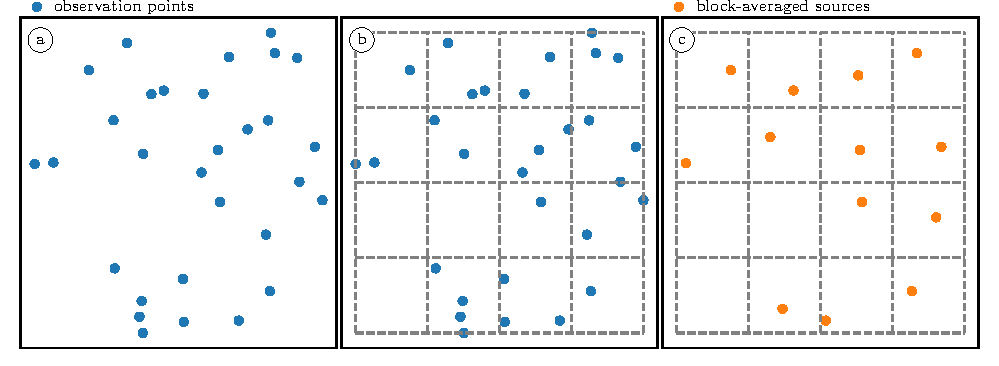
\includegraphics[width=\linewidth]{figs/block-averaged-sources-schematics.pdf}
    \caption{
        Block averaged sources.
        (a)~Given a set of observation points
        (b)~we divide the survey region on blocks of equal size and compute the
            median location of the observation points that fall inside each
            block.
        (c)~A source point is located beneath each block averaged coordinate.
            The number of point sources could be less or equal to the number of
            observation points. No source is located beneath unpopulated
            blocks.
    }
    \label{fig:block-averaged-sources}
\end{figure*}

\begin{figure*}
    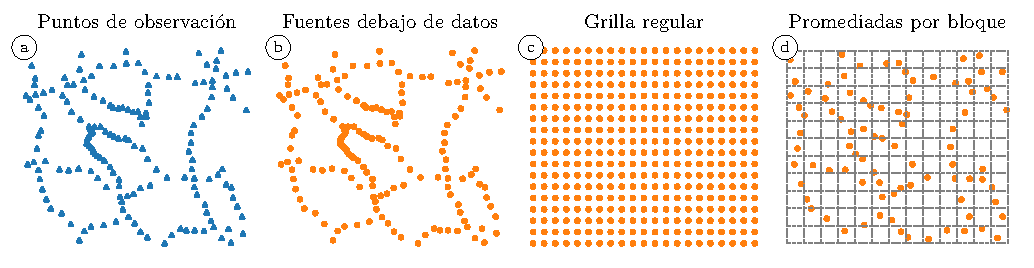
\includegraphics[width=\linewidth]{figs/source-layouts-schematics.pdf}
    \caption{
        Source layouts.
        (a) Set of \SourceLayoutsSchematicsObservations{} synthetic observation
            points that resemble a ground survey.
        (b) Location of the \SourceLayoutsSchematicsSourceBelowData{} sources
            obtained through the \emph{sources below data} layout.
        (c) Location of the \SourceLayoutsSchematicsBlockAveragedSources{}
            sources obtained through the \emph{block averaged sources} layout.
        (d) Location of the \SourceLayoutsSchematicsGridSources{} sources
            obtained through the \emph{grid sources} layout.
    }
    \label{fig:source-layouts-schematics}
\end{figure*}


\subsubsection{Depth of sources}

The depth of the point sources can be chosen following different criteria.
Deep sources generate low frequencies, while shallow ones generate high
frequencies (cite).
The simplest option is to locate all sources at the same depth, which we will
call \emph{constant depth} in the future (see Fig.~\ref{fig:depth-types}(a)).
If the measurement were taken at significantly different altitudes, the
elevated computation points will be more distant to the sources than the lower
ones.
This may create problems on reproducing high frequencies on the elevated
points.

One possible solution is to locate each source below its corresponding
observation (or block averaged) point at a constant \emph{relative depth}
from it.
The depth of each source can be computed as the height of its corresponding
observation (or block averaged) point minus a depth parameter that assumes the
same value for all sources (see Fig.~\ref{fig:depth-types}(b)).
The sources won't be all at the same depth, but they will all be at the same
distance from their corresponding observation (or block averaged) point.

In case our survey presents heavily clustered data points on some areas, we may
want the sources below that region to be shallower in order to reproduce the
high frequencies measured by these clustered observation points.
We can propose a \emph{variable depth} approach: it locates each point source
according to the \emph{relative depth} and then subtracts a term proportional
to the mean distance to its $k$ nearest neighbour sources
(see Fig.~\ref{fig:depth-types}(c)).
So, the depth of the sources can be computed as follows:

\begin{equation}
    \begin{split}
        \textrm{depth} =
           &\textrm{data point height} - \textrm{relative depth} \\
           &- \textrm{depth factor} \cdot \textrm{mean distance}
    \end{split}
\end{equation}

\noindent where \emph{data point height} is the elevation of the corresponding
observation (or block averaged) point, \emph{mean distance} is the mean
distance to the $k$ nearest source neighbours, \emph{depth factor} and
\emph{relative depth} are parameters.
The addition of this new term will make clustered sources to be shallower than
scattered and distant sources.

Similar approaches for setting sources at depths that depend
on the distance to their nearest neighbours were already proposed by
\citet{cordell1992, guspi2004, guspi2009}.

\begin{figure*}
    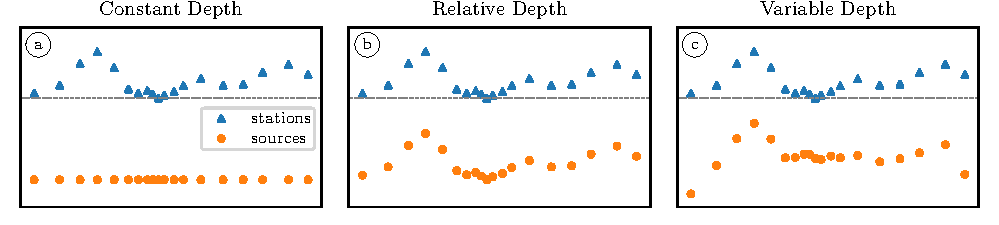
\includegraphics[width=\linewidth]{figs/depth_types.pdf}
    \caption{
        Depth types for locating point sources. We put one source beneath each
        observation point (station) using:
        (a)~a \emph{constant depth} where all sources are located at the same
           depth,
        (b)~a \emph{relative depth} where all sources are located at the same
           vertical distance from its corresponding observation point, and
        (c)~a \emph{variable depth} where the depth of the sources is
           proportional to the average distance to its neighbour sources.
           Notice how the clustered sources on (c) are relatively shallower
           than the
           other ones.
    }
    \label{fig:depth-types}
\end{figure*}

The combination of the three source layouts with the three strategies to define
the depth of the sources define seven different source distributions (see
Table~\ref{tab:source-distributions}).
The \emph{grid sources} is only compatible with the \emph{constant depth}
scheme if no further information is provided.

\begin{table*}
    \centering
    \caption{
        Source distributions as combinations of source layouts and depth
        strategies.
    }
    \label{tab:source-distributions}
    \begin{tabular}{lccc}
        & Source below data & Block averaged sources & Grid sources \\ \hline
        Constant depth & $\checkmark$ & $\checkmark$ & $\checkmark$ \\
        Relative depth & $\checkmark$ & $\checkmark$ & $\times$     \\
        Variable depth & $\checkmark$ & $\checkmark$ & $\times$     \\
    \end{tabular}
\end{table*}
%%%%%%%%%%%%%%%%%%%%%%%%%%%%%%%%%%%%%%%%%%%%%%%%%%%%%%%%%%%%%%%%%%%%%%%%%%%%%%%


\section{Comparison of source distributions}

Our first goal is to to compare the performance of all source distributions
from Table~\ref{tab:source-distributions} when predicting harmonic field data
using the equivalent sources technique.
To do so we have created a synthetic model made out of prisms of different
shape and density contrasts.
The gravitational effect of this synthetic model have been computed on
a regular grid (\emph{target} grid) at a constant height and on two different
set of observation points that we will call \emph{synthetic surveys}: a ground
and an airborne survey.
The data from each synthetic survey is interpolated on the points of the
\emph{target} grid and then scored against its values.
We can then quantitatively compare how accurate is each source distribution at
predicting unobserved data on each synthetic survey and quantify the
computational load needed to do it.

\subsection{Synthetic Model}

%Describe forward model made out of prisms.
%Show prisms model?

The synthetic model is made out of \NPrisms{} prisms distributed on a region of
\ModelEasting{}$\times$\ModelNorthing{} between \ModelDepth{} deep and the zero
height plane.
Density contrast of prisms range from \ModelMinDensity{} and
\ModelMaxDensity{}.
We built deep big and thin shallow prisms for creating gravity anomalies with
long and short wavelengths, respectively.

The vertical component of the gravity acceleration generated by the synthetic
model has been computed on a regular grid of
\TargetEastingSize{}$\times$\TargetNorthingSize{} points with a spacing of
\TargetSpacing{} located \TargetHeight{} above the zero height plane
(Fig.~\ref{fig:target-grid}), using \citet{nagy2000} and \citet{nagy2002}.
We will refer to this grid as the \emph{target} grid in the future.

\begin{figure}
    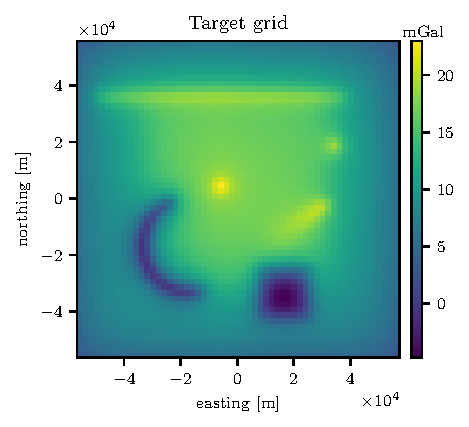
\includegraphics[width=\linewidth]{figs/target-grid.pdf}
    \caption{
        Target grid. Gravitational effect of synthetic model on a regular grid
        composed of \TargetEastingSize{}$\times$\TargetNorthingSize{} points
        with a spacing of \TargetSpacing{} located \TargetHeight{} above the
        zero height plane.
    }
    \label{fig:target-grid}
\end{figure}

\subsection{Synthetic Surveys}

In order to compare the predictive capabilities of each source distribution
under on different surveys, we created a ground and an airborne \emph{synthetic
surveys}.
For creating the synthetic ground survey we selected a portion of the Southern
Africa Gravity Data available through the
\href{https://www.ngdc.noaa.gov/mgg/gravity/gravity.html}{NOAA website}.
For the airborne survey we used a portion of the Great Britain Aeromagnetic
Survey acquired by Hunting Geology and Geophysics Ltd and Canadian Aeroservices
Ltd between 1955 and 1965 and made available by the
\href{https://www.bgs.ac.uk/products/geophysics/aeromagneticRegional.html}{
British Geological Survey (BGS)
}.

On both cases we selected only a portion of the survey and rescaled it to span
on an area of \SurveyEasting{}$\times$\SurveyNorthing{}.
The ground survey is composed by \GroundSurveyPoints{} observation points
distributed at heights ranging between \GroundSurveyMinHeight{} and
\GroundSurveyMaxHeight{} (Fig.~\ref{fig:synthetic-ground-survey}(a)).
While the airborne survey has \AirborneSurveyPoints{} points at heights between
\AirborneSurveyMinHeight{} and \AirborneSurveyMaxHeight{}.
(Fig.~\ref{fig:synthetic-ground-survey}(a)).

The vertical component of the gravity acceleration generated by the synthetic
model has been computed on both surveys.
Some Gaussian noise (with standard deviation of \SurveyNoise{}) has been added
to the effect of the synthetic model to simulate acquisition errors
(Figs.~\ref{fig:synthetic-ground-survey}(b)
and~\ref{fig:synthetic-airborne-survey}(b)).

\begin{figure}
    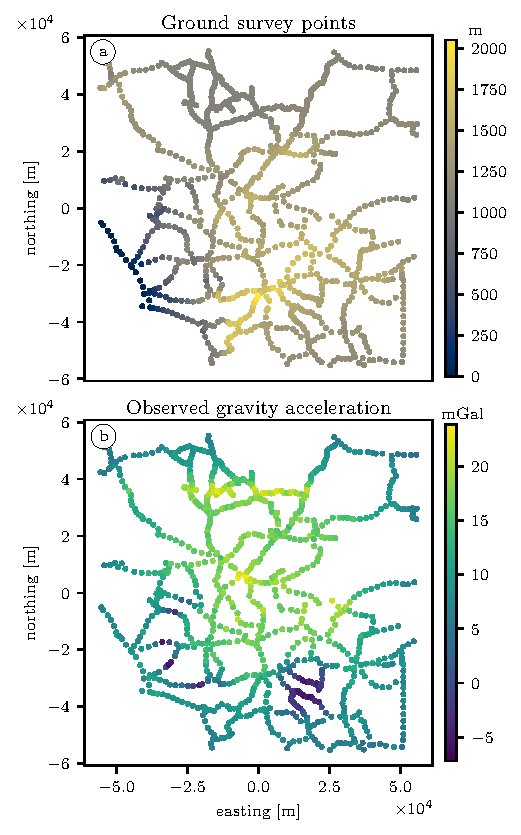
\includegraphics[width=\linewidth]{figs/ground-survey.pdf}
    \caption{
        Synthetic ground survey.
        (a)~Location of observation points. Altitude given in meters above the
            zero height plane.
        (b)~Vertical component of gravity acceleration generated by the
            synthetic model plus Gaussian noise on the ground survey
            observation points.
    }
    \label{fig:synthetic-ground-survey}
\end{figure}

\begin{figure}
    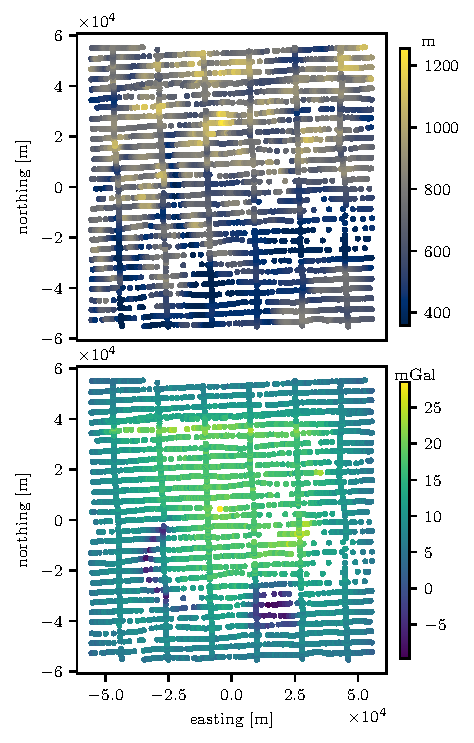
\includegraphics[width=\linewidth]{figs/airborne-survey.pdf}
    \caption{
        Synthetic airborne survey.
        (a)~Location of observation points. Altitude given in meters above the
            zero height plane.
        (b)~Vertical component of gravity acceleration generated by the
            synthetic model plus Gaussian noise on the airborne survey
            observation points.
        Based upon the Great Britain aeromagnetic data, with the permission of
        the British Geological Survey.
    }
    \label{fig:synthetic-airborne-survey}
\end{figure}

\subsection{Comparisons}

Each source distribution from Table~\ref{tab:source-distributions} needs
certain parameters in order to build the set of point sources.
The prediction capabilities of the source distribution depends on the choice of
these parameters.
For example, locating the sources beneath the data points at constant depth
needs the definition of the \emph{depth} parameter.
If the sources are set too close to the data points, the source distribution
it's very likely to over-fit the data: the measured field will be recovered, but
the predictions on unobserved locations will be very inaccurate.
Another parameter that plays an important role on the predictive capabilities
of the sources is the \emph{damping}.

On real world scenarios, choosing the values of the parameters is a challenging
task: it's not easy to determine the accuracy of the predictions without
knowing the true value of the field on unobserved locations.
This problem can be solved through cross-validation.
When working with a synthetic model, the situation is different: we can compute
the true values of harmonic field generated by the synthetic model on any
point.
Therefore, interpolating the observed data on the same points of the
\emph{target} grid and then scoring the prediction against the true values of
the \emph{target} grid constitutes an objective way to measure the predictive
accuracy of the source distribution.

In order to compare the predictive capabilities of each source distribution we
perform a parameter search to obtain the best prediction that can be achieved
by each one of them.
For each source distribution we proposed different values for each parameter
(see Tables~\ref{tab:parameters-ground-survey}
and~\ref{tab:parameters-airborne-survey}).
These parameters values are combined obtaining several \emph{set of
parameters}.
We use each set of parameters to create the sources, fit their coefficients
through least-squares and predict the field on the same points of the
\emph{target} grid.
We then \emph{score} the prediction by computing the root mean square (RMS)
between the prediction and the true values of the \emph{target} grid.
Finally, we obtain the \emph{best prediction} for each source distribution as
the one that achieves the lowest RMS.
This process is carried out on both ground and airborne synthetic surveys.
See Figure~\ref{fig:flowchart} for a graphical illustration of it.

\begin{figure}
    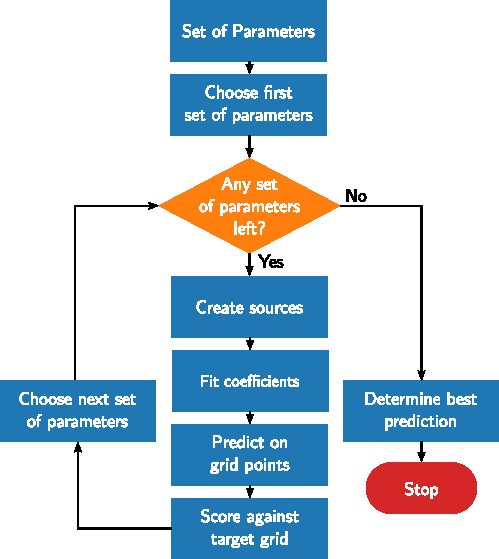
\includegraphics[width=\linewidth]{figs/flowchart.pdf}
    \caption{
        Flowchart for comparing the performance of the source distributions.
        For each source distribution we propose different values for its
        parameters (see Tables~\ref{tab:parameters-ground-survey}
        and~\ref{tab:parameters-airborne-survey}).
        These values are then combined to obtain several set of parameters
        which are iteratively submitted to the process illustrated on this
        figure.
        Finally we obtain the best prediction generated by each source
        distribution as the one that achieves the best score.
    }
    \label{fig:flowchart}
\end{figure}


Tables~\ref{tab:parameters-ground-survey}
and~\ref{tab:parameters-airborne-survey} also show the parameter combination
that produces the best prediction for each source distribution and its
corresponding RMS score, for both ground and airborne synthetic surveys,
respectively.
Figures~\ref{fig:ground-survey-differences}
and~\ref{fig:airborne-survey-differences} show the differences between the
target grid and the best prediction achieved by each source distribution, for
both ground and airborne synthetic surveys, respectively.

\begin{figure*}
    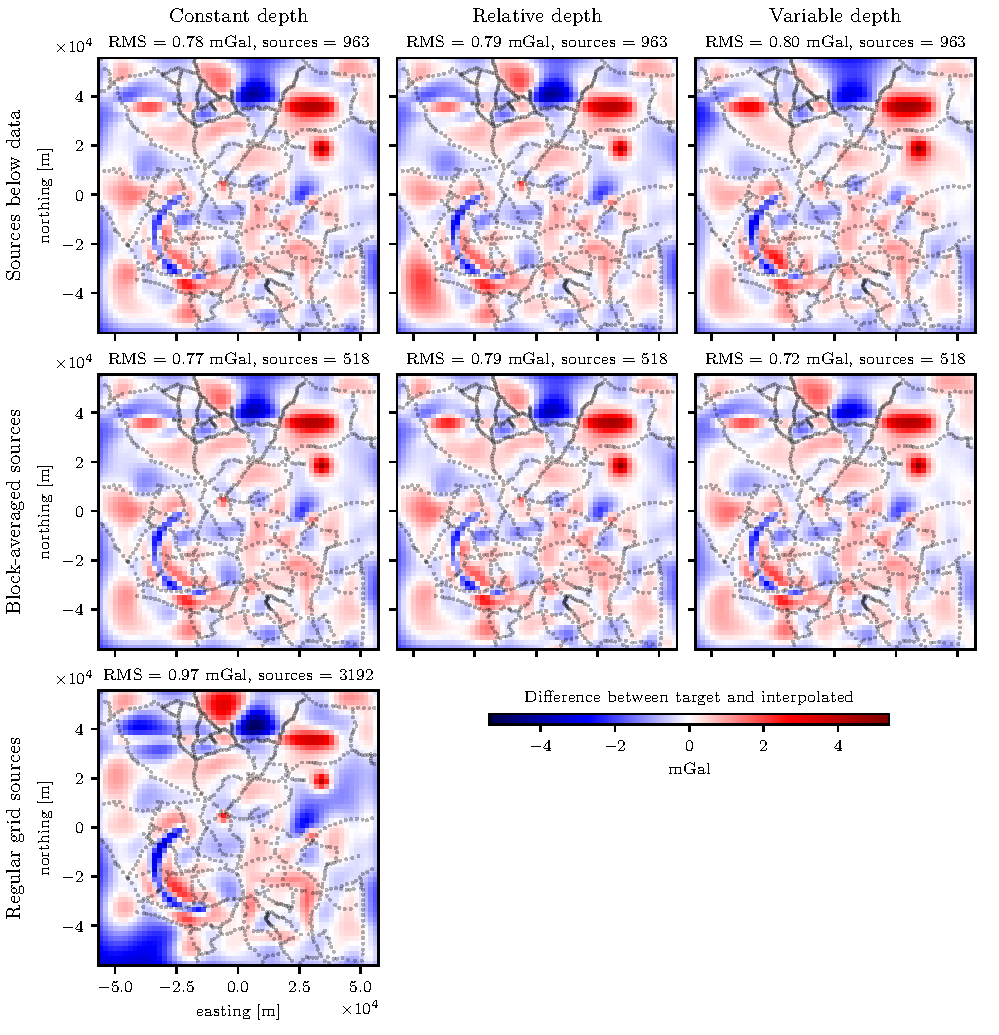
\includegraphics[width=\linewidth]{figs/ground_survey_differences.pdf}
    \caption{
        Differences between gravitational effects measured on the target grid
        and the ones produced by the best prediction made by each source
        distribution based on the synthetic ground survey.
    }
    \label{fig:ground-survey-differences}
\end{figure*}

\begin{figure*}
    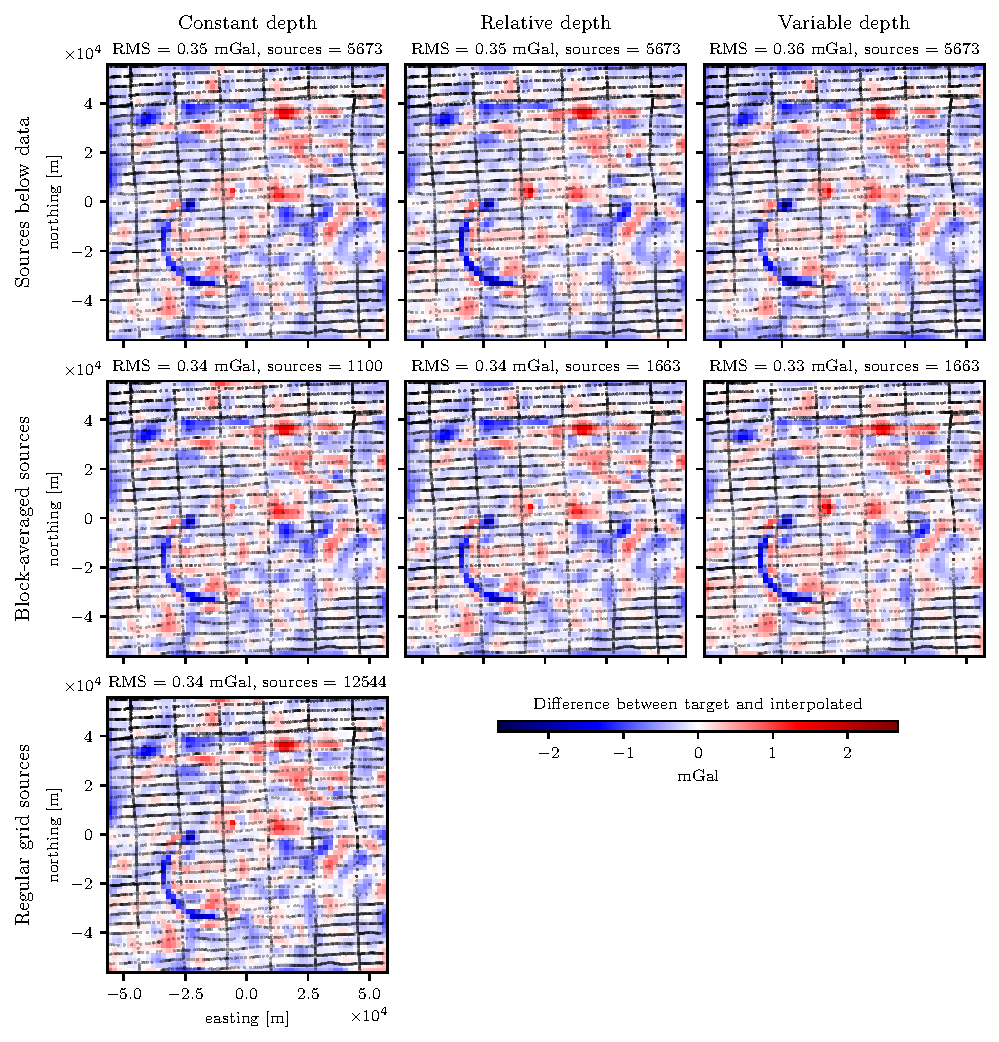
\includegraphics[width=\linewidth]{figs/airborne_survey_differences.pdf}
    \caption{
        Differences between gravitational effects measured on the target grid
        and the ones produced by the best prediction made by each source
        distribution based on the synthetic airborne survey.
    }
    \label{fig:airborne-survey-differences}
\end{figure*}



\subsection{Discussion}

Figures~\ref{fig:ground-survey-differences}
and~\ref{fig:airborne-survey-differences} show that all source distributions
produce accurate predictions, both for the ground and airborne survey.
The RMS scores don't show significant difference, so we can only conclude
that all the source distributions are able to produce comparable predictions.
Nevertheless, the \emph{block averaged sources} make use of less sources to
produce this predictions, what would reduce the computational load needed to
fit the sources coefficients and finally compute the actual prediction.

The RMS doesn't seem to depend on the choice of the depth strategy used to
locate the equivalent sources.
At first glance, the choice of a depth strategy doesn't seem to impact the
computational needs.
Nevertheless, when trying to find the set of parameters that produce the most
accurate predictions through a method like cross-validation, we need to fit the
source coefficients one time per every possible combination of parameters.
A depth strategy like the \emph{variable depth} needs a higher number of
parameters (depth, depth factor, K nearest) than \emph{constant depth} or
\emph{relative depth} (which takes only a depth parameter).
The addition of these new parameters makes the search of the best set more
computationally expensive: more parameters means increasing the dimensions of
the parameters space and thus increasing the number of possible combinations.
Therefore we would be more prone to choose a \emph{constant depth} or
a \emph{relative depth} when dealing with very large datasets in order to save
some computation time.

%%%%%%%%%%%%%%%%%%%%%%%%%%%%%%%%%%%%%%%%%%%%%%%%%%%%%%%%%%%%%%%%%%%%%%%%%%%%%%%

\section{Performance of gradient-boosted equivalent sources}

Our second goal is to assess the accuracy of the predictions achieved by the
gradient boosting algorithm while registering its performance by comparison
with the non-boosted equivalent sources.


\subsection{Window size}
\label{sec:window_size}

One factor that plays an important role on the performance of the gradient
boosted equivalent sources is the size of the overlapping windows used to create
each set of equivalent sources.
The size of the windows controls the size of the Jacobian matrices
$\tilde{\mathbf{A}_k}$: smaller windows create smaller Jacobian matrices.
Thus, using smaller windows will reduce the amount of computer memory needed to
fit the source coefficients.
Nevertheless, smaller windows may produce less accurate predictions because
their inability to achieve the global minimum of the misfit from
equation~\ref{eq:misfit-unscaled}.
Besides, the window size might also impact on the computation time needed to
fit the source coefficients: smaller windows will generate simpler least-square
problems which are easier to solve, but they will also create more iterations.

We want to assess how the size of the overlapping windows impacts both the
accuracy of the predictions and the computation time needed to fit the source
coefficients in comparison with the performance of the non-boosted equivalent
sources.

We applied the gradient boosted equivalent sources to interpolate the synthetic
airborne survey on the same points of the target grid.
We selected several window sizes to assess how accuracy and performance depend
on that variable.
For each window size we gridded the synthetic data using block-averaged sources
with a spacing of
\SI{\BestAirborneBlockAveragedSourcesRelativeDepthSpacing}{\meter},
a relative depth of
\SI{\BestAirborneBlockAveragedSourcesRelativeDepthDepth}{\meter}, an overlap
of 50\%, and with different values of damping.
Then we compared the resulting interpolations with the target grid in order to
get the best prediction for each window size and the damping value used to
obtain it.

Using the best set of parameters for each window size, we registered the
achieved RMS against the values of the target grid and the time needed to fit
the sources coefficients.
In order to avoid any errors introduced by the way windows are shuffled, the
RMS for each window size was obtained as the mean RMS achieved by using
different random seeds.


\subsection{Overlapping}

Another factor that plays an important role on the performance of the gradient
boosted equivalent sources is the amount of overlap between adjacent windows.
The previous choice of 50\% showed to be sufficiently good to achieve
acceptable accuracy, although a deeper study should be carried out to assess
how the amount of overlap impacts both accuracy and fitting time.

We interpolated the synthetic airborne survey using the gradient boosted
equivalent sources on the same points of the target grid.
The interpolations were carried out using different amount of overlap, from
0\% to 0.95\% with a step size of 0.05\%.
For each overlap we gridded the synthetic data using block-averaged sources
with a spacing of
\SI{\BestAirborneBlockAveragedSourcesRelativeDepthSpacing}{\meter},
a relative depth of
\SI{\BestAirborneBlockAveragedSourcesRelativeDepthDepth}{\meter},
a window size of \BoostOverlappingWindowSize, and with different
values of damping.
Then we compared the resulting interpolations with the target grid in order to
get the best prediction for each overlap and the damping value used to
obtain it.

Using the best set of parameters for each overlap, we registered the achieved
RMS against the values of the target grid and the time needed to fit the
sources coefficients.
The RMS was obtained as the mean RMS achieved by using different random seeds
as we did on~\ref{sec:window_size}.


%%%%%%%%%%%%%%%%%%%%%%%%%%%%%%%%%%%%%%%%%%%%%%%%%%%%%%%%%%%%%%%%%%%%%%%%%%%%%%%

\section{Gridding Australia gravity data}

%%%%%%%%%%%%%%%%%%%%%%%%%%%%%%%%%%%%%%%%%%%%%%%%%%%%%%%%%%%%%%%%%%%%%%%%%%%%%%%

\section{Conclusions}

%%%%%%%%%%%%%%%%%%%%%%%%%%%%%%%%%%%%%%%%%%%%%%%%%%%%%%%%%%%%%%%%%%%%%%%%%%%%%%%

\section{Acknowledgements}

We are indebted to the developers and maintainers of the open-source software
without which this work would not have been possible.

The synthetic airborne survey was based upon the Great Britain aeromagnetic
data, reproduced with the permission of the British Geological Survey
$\textcopyright$UKRI\@.
All rights reserved.

%%%%%%%%%%%%%%%%%%%%%%%%%%%%%%%%%%%%%%%%%%%%%%%%%%%%%%%%%%%%%%%%%%%%%%%%%%%%%%%

\appendix

\section{Source distributions parameters}

\begin{table*}
    \centering
    \caption{
        Parameters used with each source distribution when gridding the
        synthetic ground survey. The table also contains the set of parameters
        that generates the best prediction for each source distribution and its
        corresponding RMS score (in mGal).
    }
    \label{tab:parameters-ground-survey}
    \begin{tabular}{c c l c c c}
        \textbf{Source layout}
            & \textbf{Depth type}
            & \multicolumn{1}{c}{\textbf{Parameters}}
            & \textbf{Values}
            & \textbf{Best}
            & \textbf{RMS} \\
        \toprule

        \multirow{8}{*}{Source Below Data}
            & \multirow{2}{*}{Constant}
                & Depth (m)
                & \GroundSourceBelowDataConstantDepthDepth
                & \BestGroundSourceBelowDataConstantDepthDepth
                & \multirow{2}{*}{
                    \BestGroundSourceBelowDataConstantDepthRms
                  } \\
            &
                & Damping
                & \GroundSourceBelowDataConstantDepthDamping
                & \BestGroundSourceBelowDataConstantDepthDamping
                & \\
            \cmidrule{2-6}
            & \multirow{2}{*}{Relative}
                & Depth (m)
                & \GroundSourceBelowDataRelativeDepthDepth
                & \BestGroundSourceBelowDataRelativeDepthDepth
                & \multirow{2}{*}{
                    \BestGroundSourceBelowDataRelativeDepthRms
                  } \\
            &
                & Damping
                & \GroundSourceBelowDataRelativeDepthDamping
                & \BestGroundSourceBelowDataRelativeDepthDamping
                & \\
            \cmidrule{2-6}
            & \multirow{4}{*}{Variable}
                & Depth (m)
                & \GroundSourceBelowDataVariableDepthDepth
                & \BestGroundSourceBelowDataVariableDepthDepth
                & \multirow{4}{*}{
                    \BestGroundSourceBelowDataVariableDepthRms
                  } \\
            &
                & Depth factor
                & \GroundSourceBelowDataVariableDepthDepthFactor
                & \BestGroundSourceBelowDataVariableDepthDepthFactor
                & \\
            &
                & K nearest
                & \GroundSourceBelowDataVariableDepthKNearest
                & \BestGroundSourceBelowDataVariableDepthKNearest
                & \\
            &
                & Damping
                & \GroundSourceBelowDataVariableDepthDamping
                & \BestGroundSourceBelowDataVariableDepthDamping
                & \\
        \midrule

        \multirow{11}{*}{Block Averaged Sources}
            & \multirow{3}{*}{Constant}
                & Depth (m)
                & \GroundBlockAveragedSourcesConstantDepthDepth
                & \BestGroundBlockAveragedSourcesConstantDepthDepth
                & \multirow{3}{*}{
                    \BestGroundBlockAveragedSourcesConstantDepthRms
                  } \\
            &
                & Spacing (m)
                & \GroundBlockAveragedSourcesConstantDepthSpacing
                & \BestGroundBlockAveragedSourcesConstantDepthSpacing
                & \\
            &
                & Damping
                & \GroundBlockAveragedSourcesConstantDepthDamping
                & \BestGroundBlockAveragedSourcesConstantDepthDamping
                & \\
            \cmidrule{2-6}
            & \multirow{3}{*}{Relative}
                & Depth (m)
                & \GroundBlockAveragedSourcesRelativeDepthDepth
                & \BestGroundBlockAveragedSourcesRelativeDepthDepth
                & \multirow{3}{*}{
                    \BestGroundBlockAveragedSourcesRelativeDepthRms
                  } \\
            &
                & Spacing (m)
                & \GroundBlockAveragedSourcesRelativeDepthSpacing
                & \BestGroundBlockAveragedSourcesRelativeDepthSpacing
                & \\
            &
                & Damping
                & \GroundBlockAveragedSourcesRelativeDepthDamping
                & \BestGroundBlockAveragedSourcesRelativeDepthDamping
                & \\
            \cmidrule{2-6}
            & \multirow{5}{*}{Variable}
                & Depth (m)
                & \GroundBlockAveragedSourcesVariableDepthDepth
                & \BestGroundBlockAveragedSourcesVariableDepthDepth
                & \multirow{5}{*}{
                    \BestGroundBlockAveragedSourcesVariableDepthRms
                  } \\
            &
                & Depth factor
                & \GroundBlockAveragedSourcesVariableDepthDepthFactor
                & \BestGroundBlockAveragedSourcesVariableDepthDepthFactor
                & \\
            &
                & K nearest
                & \GroundBlockAveragedSourcesVariableDepthKNearest
                & \BestGroundBlockAveragedSourcesVariableDepthKNearest
                & \\
            &
                & Spacing (m)
                & \GroundBlockAveragedSourcesVariableDepthSpacing
                & \BestGroundBlockAveragedSourcesVariableDepthSpacing
                & \\
            &
                & Damping
                & \GroundBlockAveragedSourcesVariableDepthDamping
                & \BestGroundBlockAveragedSourcesVariableDepthDamping
                & \\
        \midrule

        \multirow{4}{*}{Grid Sources}
            & \multirow{4}{*}{Constant}
                & Depth (m)
                & \GroundGridSourcesConstantDepthDepth
                & \BestGroundGridSourcesConstantDepthDepth
                & \multirow{4}{*}{
                    \BestGroundGridSourcesConstantDepthRms
                  } \\
            &
                & Spacing (m)
                & \GroundGridSourcesConstantDepthSpacing
                & \BestGroundGridSourcesConstantDepthSpacing
                & \\
            &
                & Damping
                & \GroundGridSourcesConstantDepthDamping
                & \BestGroundGridSourcesConstantDepthDamping
                & \\
    \end{tabular}
\end{table*}

\begin{table*}
    \centering
    \caption{
        Parameters used with each source distribution when gridding the
        synthetic airborne survey. The table also contains the set of
        parameters that generates the best prediction for each source
        distribution and its corresponding RMS score (in mGal).
    }
    \label{tab:parameters-airborne-survey}
    \begin{tabular}{c c l c c c}
        \textbf{Source layout}
            & \textbf{Depth type}
            & \multicolumn{1}{c}{\textbf{Parameters}}
            & \textbf{Values}
            & \textbf{Best}
            & \textbf{RMS} \\
        \toprule

        \multirow{8}{*}{Source Below Data}
            & \multirow{2}{*}{Constant}
                & Depth (m)
                & \AirborneSourceBelowDataConstantDepthDepth
                & \BestAirborneSourceBelowDataConstantDepthDepth
                & \multirow{2}{*}{
                    \BestAirborneSourceBelowDataConstantDepthRms
                  } \\
            &
                & Damping
                & \AirborneSourceBelowDataConstantDepthDamping
                & \BestAirborneSourceBelowDataConstantDepthDamping
                & \\
            \cmidrule{2-6}
            & \multirow{2}{*}{Relative}
                & Depth (m)
                & \AirborneSourceBelowDataRelativeDepthDepth
                & \BestAirborneSourceBelowDataRelativeDepthDepth
                & \multirow{2}{*}{
                    \BestAirborneSourceBelowDataRelativeDepthRms
                  } \\
            &
                & Damping
                & \AirborneSourceBelowDataRelativeDepthDamping
                & \BestAirborneSourceBelowDataRelativeDepthDamping
                & \\
            \cmidrule{2-6}
            & \multirow{4}{*}{Variable}
                & Depth (m)
                & \AirborneSourceBelowDataVariableDepthDepth
                & \BestAirborneSourceBelowDataVariableDepthDepth
                & \multirow{4}{*}{
                    \BestAirborneSourceBelowDataVariableDepthRms
                  } \\
            &
                & Depth factor
                & \AirborneSourceBelowDataVariableDepthDepthFactor
                & \BestAirborneSourceBelowDataVariableDepthDepthFactor
                & \\
            &
                & K nearest
                & \AirborneSourceBelowDataVariableDepthKNearest
                & \BestAirborneSourceBelowDataVariableDepthKNearest
                & \\
            &
                & Damping
                & \AirborneSourceBelowDataVariableDepthDamping
                & \BestAirborneSourceBelowDataVariableDepthDamping
                & \\
        \midrule

        \multirow{11}{*}{Block Averaged Sources}
            & \multirow{3}{*}{Constant}
                & Depth (m)
                & \AirborneBlockAveragedSourcesConstantDepthDepth
                & \BestAirborneBlockAveragedSourcesConstantDepthDepth
                & \multirow{3}{*}{
                    \BestAirborneBlockAveragedSourcesConstantDepthRms
                  } \\
            &
                & Spacing (m)
                & \AirborneBlockAveragedSourcesConstantDepthSpacing
                & \BestAirborneBlockAveragedSourcesConstantDepthSpacing
                & \\
            &
                & Damping
                & \AirborneBlockAveragedSourcesConstantDepthDamping
                & \BestAirborneBlockAveragedSourcesConstantDepthDamping
                & \\
            \cmidrule{2-6}
            & \multirow{3}{*}{Relative}
                & Depth (m)
                & \AirborneBlockAveragedSourcesRelativeDepthDepth
                & \BestAirborneBlockAveragedSourcesRelativeDepthDepth
                & \multirow{3}{*}{
                    \BestAirborneBlockAveragedSourcesRelativeDepthRms
                  } \\
            &
                & Spacing (m)
                & \AirborneBlockAveragedSourcesRelativeDepthSpacing
                & \BestAirborneBlockAveragedSourcesRelativeDepthSpacing
                & \\
            &
                & Damping
                & \AirborneBlockAveragedSourcesRelativeDepthDamping
                & \BestAirborneBlockAveragedSourcesRelativeDepthDamping
                & \\
            \cmidrule{2-6}
            & \multirow{5}{*}{Variable}
                & Depth (m)
                & \AirborneBlockAveragedSourcesVariableDepthDepth
                & \BestAirborneBlockAveragedSourcesVariableDepthDepth
                & \multirow{5}{*}{
                    \BestAirborneBlockAveragedSourcesVariableDepthRms
                  } \\
            &
                & Depth factor
                & \AirborneBlockAveragedSourcesVariableDepthDepthFactor
                & \BestAirborneBlockAveragedSourcesVariableDepthDepthFactor
                & \\
            &
                & K nearest
                & \AirborneBlockAveragedSourcesVariableDepthKNearest
                & \BestAirborneBlockAveragedSourcesVariableDepthKNearest
                & \\
            &
                & Spacing (m)
                & \AirborneBlockAveragedSourcesVariableDepthSpacing
                & \BestAirborneBlockAveragedSourcesVariableDepthSpacing
                & \\
            &
                & Damping
                & \AirborneBlockAveragedSourcesVariableDepthDamping
                & \BestAirborneBlockAveragedSourcesVariableDepthDamping
                & \\
        \midrule

        \multirow{4}{*}{Grid Sources}
            & \multirow{4}{*}{Constant}
                & Depth (m)
                & \AirborneGridSourcesConstantDepthDepth
                & \BestAirborneGridSourcesConstantDepthDepth
                & \multirow{4}{*}{
                    \BestAirborneGridSourcesConstantDepthRms
                  } \\
            &
                & Spacing (m)
                & \AirborneGridSourcesConstantDepthSpacing
                & \BestAirborneGridSourcesConstantDepthSpacing
                & \\
            &
                & Damping
                & \AirborneGridSourcesConstantDepthDamping
                & \BestAirborneGridSourcesConstantDepthDamping
                & \\
    \end{tabular}
\end{table*}

%%%%%%%%%%%%%%%%%%%%%%%%%%%%%%%%%%%%%%%%%%%%%%%%%%%%%%%%%%%%%%%%%%%%%%%%%%%%%%%

\bibliographystyle{humannat}
\bibliography{references}

\end{document}
